\documentclass[a4paper,12pt]{article}

% Import the deliverable package from the common directory.
\usepackage{../common/deliverable}

% Tell LaTeX where to find graphics files.
\graphicspath{{../common/logos/}{./figures/}{../}}

\usepackage{xspace}
\usepackage{listings}
\usepackage{amsmath}
\usepackage{float}
\usepackage{amssymb}

\lstset{
    language=C++,
    basicstyle=\ttfamily\scriptsize,
    keywordstyle=\color{blue},
    commentstyle=\color{gray},
    stringstyle=\color{red},
    breaklines=true,
    frame=single,
    numbers=left,
    numberstyle=\tiny,
    showstringspaces=false,
    columns=fullflexible
}

\setdeliverableNumber{1.8}

\begin{document}

\maketitlepage{Polygonal discretization in deal.II -- II}

\newpage

\begin{deliverableTable}
    \tableEntry{Deliverable title}{Polygonal discretization in deal.II -- II}
    \tableEntry{Deliverable number}{D1.8}
    \tableEntry{Deliverable version}{v0.1 (draft)}
    \tableEntry{Date of delivery}{July 31, 2026}
    \tableEntry{Actual date of delivery}{Draft prepared July 16, 2026}
    % Check the nature against the Grant Agreement before submission.
    \tableEntry{Nature of deliverable}{DEM - Demonstrator, pilot, prototype}
    \tableEntry{Dissemination level}{Public}
    \tableEntry{Work Package}{WP1}
    \tableEntry{Partner responsible}{SISSA}
\end{deliverableTable}

\begin{deliverableTable}
    \tableEntry{Abstract}{This document reports the publication of an example in the deal.II Code Gallery and the submission of reusable software for discontinuous Galerkin methods on agglomerated polytopal meshes to the deal.II core library.}
    \tableEntry{Keywords}{Polygonal meshes, polytopic meshes, mesh
        agglomeration, discontinuous Galerkin methods, deal.II, Code Gallery,
        software integration}
\end{deliverableTable}

\newpage

\begin{documentControl}
    \addVersion{0.1}{16/07/2026}{Xinping Gui}{Initial draft}
\end{documentControl}

\subsection*{{Approval Details}}
Internal review and approval pending.

\subsection*{{Distribution List}}
\begin{itemize}
    \item [] - Project Coordinators (PCs)
    \item [] - Work Package Leaders (WPLs)
    \item [] - Steering Committee (SC)
    \item [] - European Commission (EC)
\end{itemize}

\vspace*{2cm}

\disclaimer

\newpage

\tableofcontents

\newpage

\section{{Introduction}}
\label{sec:introduction}

The polygonal discretization activity of dealii-X is carried out within
WP1.3, whose objective is to provide deal.II with complete and efficient
support for general-mesh discretization methods. Polygonal and polyhedral
meshes offer two complementary advantages for the applications targeted by
the project: they provide flexible representations of complex and
non-matching geometries, and they furnish natural coarse spaces for multilevel
solvers when constructed by agglomerating cells of an existing mesh. WP1.3
therefore combines the development of polygonal discretization methods with
scalable implementation, automatic coarse-grid construction, and their use in
multilevel preconditioning. The present deliverable concerns the DG and
agglomeration components of this programme.

An agglomerated polytopic mesh is obtained by grouping cells of a standard
fine triangulation into larger polygonal or polyhedral elements. By retaining
the relation between each agglomerate and its underlying fine cells, one can
represent complex element shapes while continuing to use deal.II components
for mesh handling, finite elements, linear algebra, and solvers. Such meshes
can be used directly for polytopic DG discretizations
\citep{polyDG,Antoniettihp}, or as coarse levels in multilevel methods. In
particular, the R-tree-based R3MG construction produces a nested sequence of
increasingly coarse agglomerated meshes starting from an existing fine
mesh~\citep{FEDER2025113773}. The same hierarchy has also been used to construct an agglomeration-based
multilevel preconditioner for a DG discretization of cardiac
electrophysiology~\citep{FederAfrica2026}.

%The software developments reported here contribute directly to WP1.3.1,
%through support for DG discretizations on agglomerated meshes, and to
%WP1.3.3, through the automatic construction of nested polygonal grid
%hierarchies. The proposed core framework also supports fully distributed
%triangulations, thereby contributing to the parallelization objectives of
%WP1.3.2. Moreover, the R-tree-based coarsening strategy has already been
%employed within \texttt{Polydeal} to construct an agglomeration-based
%multilevel preconditioner for a DG discretization of cardiac
%electrophysiology~\citep{FederAfrica2026}, providing a concrete realization of
%the objectives of WP1.3.4. The resulting grid hierarchies and finite element
%interfaces also provide reusable ingredients for the multiphysics
%preconditioning activities envisaged in WP1.3.5, although that broader
%integration is beyond the scope of this deliverable.

Deliverable D1.5 introduced the external \texttt{Polydeal} library and
described a Poisson tutorial on agglomerated polytopic meshes. Deliverable
D1.7 subsequently reported the testing and validation of the module, the
opening of a separate contribution to the deal.II Code Gallery, and the
ongoing refactoring of reusable components for possible integration into
deal.II. The present deliverable reports the subsequent upstream software
results. A new, self-contained agglomeration-based Poisson example, distinct
from the tutorial described in D1.5, has been developed and published in the
official deal.II Code Gallery to provide a clear presentation of the
polygonal DG workflow. In parallel, a reusable framework for DG
discretizations on agglomerated polygonal and polyhedral meshes has been
submitted to the deal.II core library through pull request \#19891. The Code
Gallery program provides a user-facing demonstrator, whereas the core-library
submission provides the general-purpose software components intended for reuse
in other applications.

%\section{{Introduction}}
%\label{sec:introduction}
%
%The dealii-X polygonal discretization activity is defined in WP1.3. It was
%established to address the lack of complete and efficient implementations of
%polygonal discretization methods in mainstream finite element libraries. Its
%overall objective is to integrate general-mesh discretization capabilities
%into deal.II, thereby enabling more flexible meshing of complex geometries and
%the use of general polygonal grids as coarse spaces and preconditioners for
%multiscale problems.
%
%The present deliverable focuses on two activities. WP1.3.1 enables polygonal
%discretization methods, whereas WP1.3.3 constructs coarse polygonal grid
%hierarchies automatically. The resulting software also provides building
%blocks for WP1.3.4, which concerns agglomeration-based geometric multigrid. The
%remaining WP1.3 activities are outside the scope of this deliverable.
%
%An agglomerated polytopic mesh is obtained by grouping cells of a standard
%fine triangulation into larger polygonal or polyhedral elements. This makes it
%possible to represent complex element shapes while continuing to use deal.II
%components for mesh handling, finite elements, linear algebra, and solvers.
%Such meshes are useful not only as computational meshes for polytopic DG
%methods~\citep{polyDG,Antoniettihp}, but also as coarse levels in multilevel
%solvers. In particular, the R-tree-based R3MG construction provides a sequence
%of increasingly coarse agglomerated meshes starting from an existing fine
%mesh~\citep{FEDER2025113773}.
%
%Deliverable D1.5 introduced the external \texttt{Polydeal} library and
%described a Poisson tutorial on agglomerated polytopic meshes. D1.7
%subsequently reported the testing and validation of the module, the opening of
%Code Gallery pull request \#233, and the ongoing refactoring of reusable
%components for submission to deal.II. The present deliverable records the next stage of this work. A separate,
%self-contained agglomeration-based Poisson example was developed for the
%official deal.II Code Gallery to provide a clearer presentation of the
%polygonal DG workflow. In parallel, a reusable framework supporting DG
%discretizations on agglomerated polygonal and polyhedral meshes was submitted
%to the deal.II core library through pull request \#19891.
%
%
%%The present deliverable records the next
%%stage of this work: the tutorial has been accepted and published as an
%%official deal.II Code Gallery program, and a reusable framework supporting DG
%%discretizations on agglomerated polygonal and polyhedral meshes has been
%%submitted to the deal.II core library through pull request \#19891.
%

\subsection{{Purpose of the Document}}

The purpose of this document is to describe how the polygonal discretization
capabilities developed in WP1.3 are made available within the deal.II
environment. It presents an agglomeration-based Poisson example that starts
from a conventional fine triangulation, constructs a polytopic mesh, and
solves the resulting problem using a symmetric interior penalty discontinuous
Galerkin method. The example provides users with a reproducible introduction
to polygonal DG discretizations and illustrates both METIS- and R-tree-based
agglomeration strategies.

The document also presents the reusable software framework developed behind
the example and proposed for integration into the deal.II core library. The
framework provides data structures and interfaces for defining and traversing
agglomerates, distributing degrees of freedom, constructing sparsity patterns,
and evaluating finite element quantities over agglomerated cells and their
interfaces. By separating these operations from the problem-specific
assembly, the proposed implementation can be reused in other DG applications
and provides the basic infrastructure required for coarse polygonal grid
hierarchies and agglomeration-based multilevel solvers.


\section{{Official deal.II Code Gallery program}}
\label{sec:code_gallery}

\subsection{{The public program}}

The published program is available at
\begin{center}
\url{https://dealii.org/developer/doxygen/deal.II/code_gallery_agglomeration_poisson.html}.
\end{center}
It is a self-contained Code Gallery example entitled \emph{An
agglomeration-based solver for the Poisson problem}. The program solves
\begin{equation}
    \begin{aligned}
        -\Delta u &= f && \text{in } \Omega,\\
                 u &= g_D && \text{on } \partial\Omega,
    \end{aligned}
\end{equation}
with a symmetric interior penalty discontinuous Galerkin method on an
agglomerated polytopic mesh.

Starting from a standard deal.II triangulation, the program groups fine cells
into agglomerates. The program demonstrates graph partitioning with
\texttt{METIS} and a geometric R-tree construction. The METIS algorithm is
described in~\citep{METIS}. The R-tree construction also generates a hierarchy
of successively coarser agglomerated meshes. The program then distributes DG
degrees of freedom on the agglomerates, constructs the sparsity pattern,
assembles cell and interface terms, solves the linear system, computes errors,
and exports the mesh and solution for visualization.

The official page contains the complete program description and source code,
examples of the generated polytopic meshes, comparisons between the two
agglomeration strategies, convergence results in the $L^2$ and broken
$H^1$ errors, and construction-time measurements.

The submission and review history is recorded in two Code Gallery pull
requests. The complete \texttt{agglomeration\_poisson} program, including its
source and build files, user documentation, and numerical results, was
submitted through
\href{https://github.com/dealii/code-gallery/pull/233}
{dealii/code-gallery pull request \#233} and merged on March 31, 2026. A
subsequent
\href{https://github.com/dealii/code-gallery/pull/244}
{pull request \#244}, merged on May 1, 2026, corrected the rendering and layout
of the figures and made related documentation-formatting adjustments. The resulting user-facing documentation is the official Code
Gallery page cited above.


\subsection{{Test case, and representative output}}

The Code Gallery program considers the Poisson problem on the unit square
$\Omega=(0,1)^2$. The numerical test is based on the manufactured exact
solution
\begin{equation}
    u_{\mathrm{ex}}(x,y)
    =
    \sin(\pi x)\sin(\pi y),
\end{equation}
with the corresponding right-hand side
\begin{equation}
    f(x,y)
    =
    2\pi^2\sin(\pi x)\sin(\pi y).
\end{equation}
The Dirichlet boundary condition is obtained from the trace of the exact
solution. Since $u_{\mathrm{ex}}=0$ on $\partial\Omega$, homogeneous
Dirichlet data are prescribed. 

The computation starts from an unstructured mesh of the unit square, followed
by five global refinement steps. The cells of the resulting fine mesh are
then grouped into agglomerated polytopic elements using either METIS
partitioning or the R-tree-based construction. The numerical problem is
discretized using the symmetric interior penalty discontinuous Galerkin
method, with penalty constant $C_{\sigma}=10$.

The program subsequently distributes the DG degrees of freedom, assembles and
solves the discrete problem, computes the $L^2$ and broken $H^1$ errors, and
exports both the agglomerated meshes and the numerical solution for
visualization. Figure~\ref{fig:code_gallery_meshes} compares the meshes
obtained with 91 and 364 agglomerates. METIS produces graph-based partitions,
whereas the R-tree strategy generates geometry-driven agglomerates associated
with the spatial hierarchy.

\begin{figure}[H]
    \centering

    \begin{minipage}[t]{0.47\textwidth}
        \centering
        
\includegraphics[width=\linewidth]{polygonmetis_91}
        \par\smallskip
        {\small (a) METIS, 91 agglomerates}
    \end{minipage}
    \hfill
    \begin{minipage}[t]{0.47\textwidth}
        \centering
        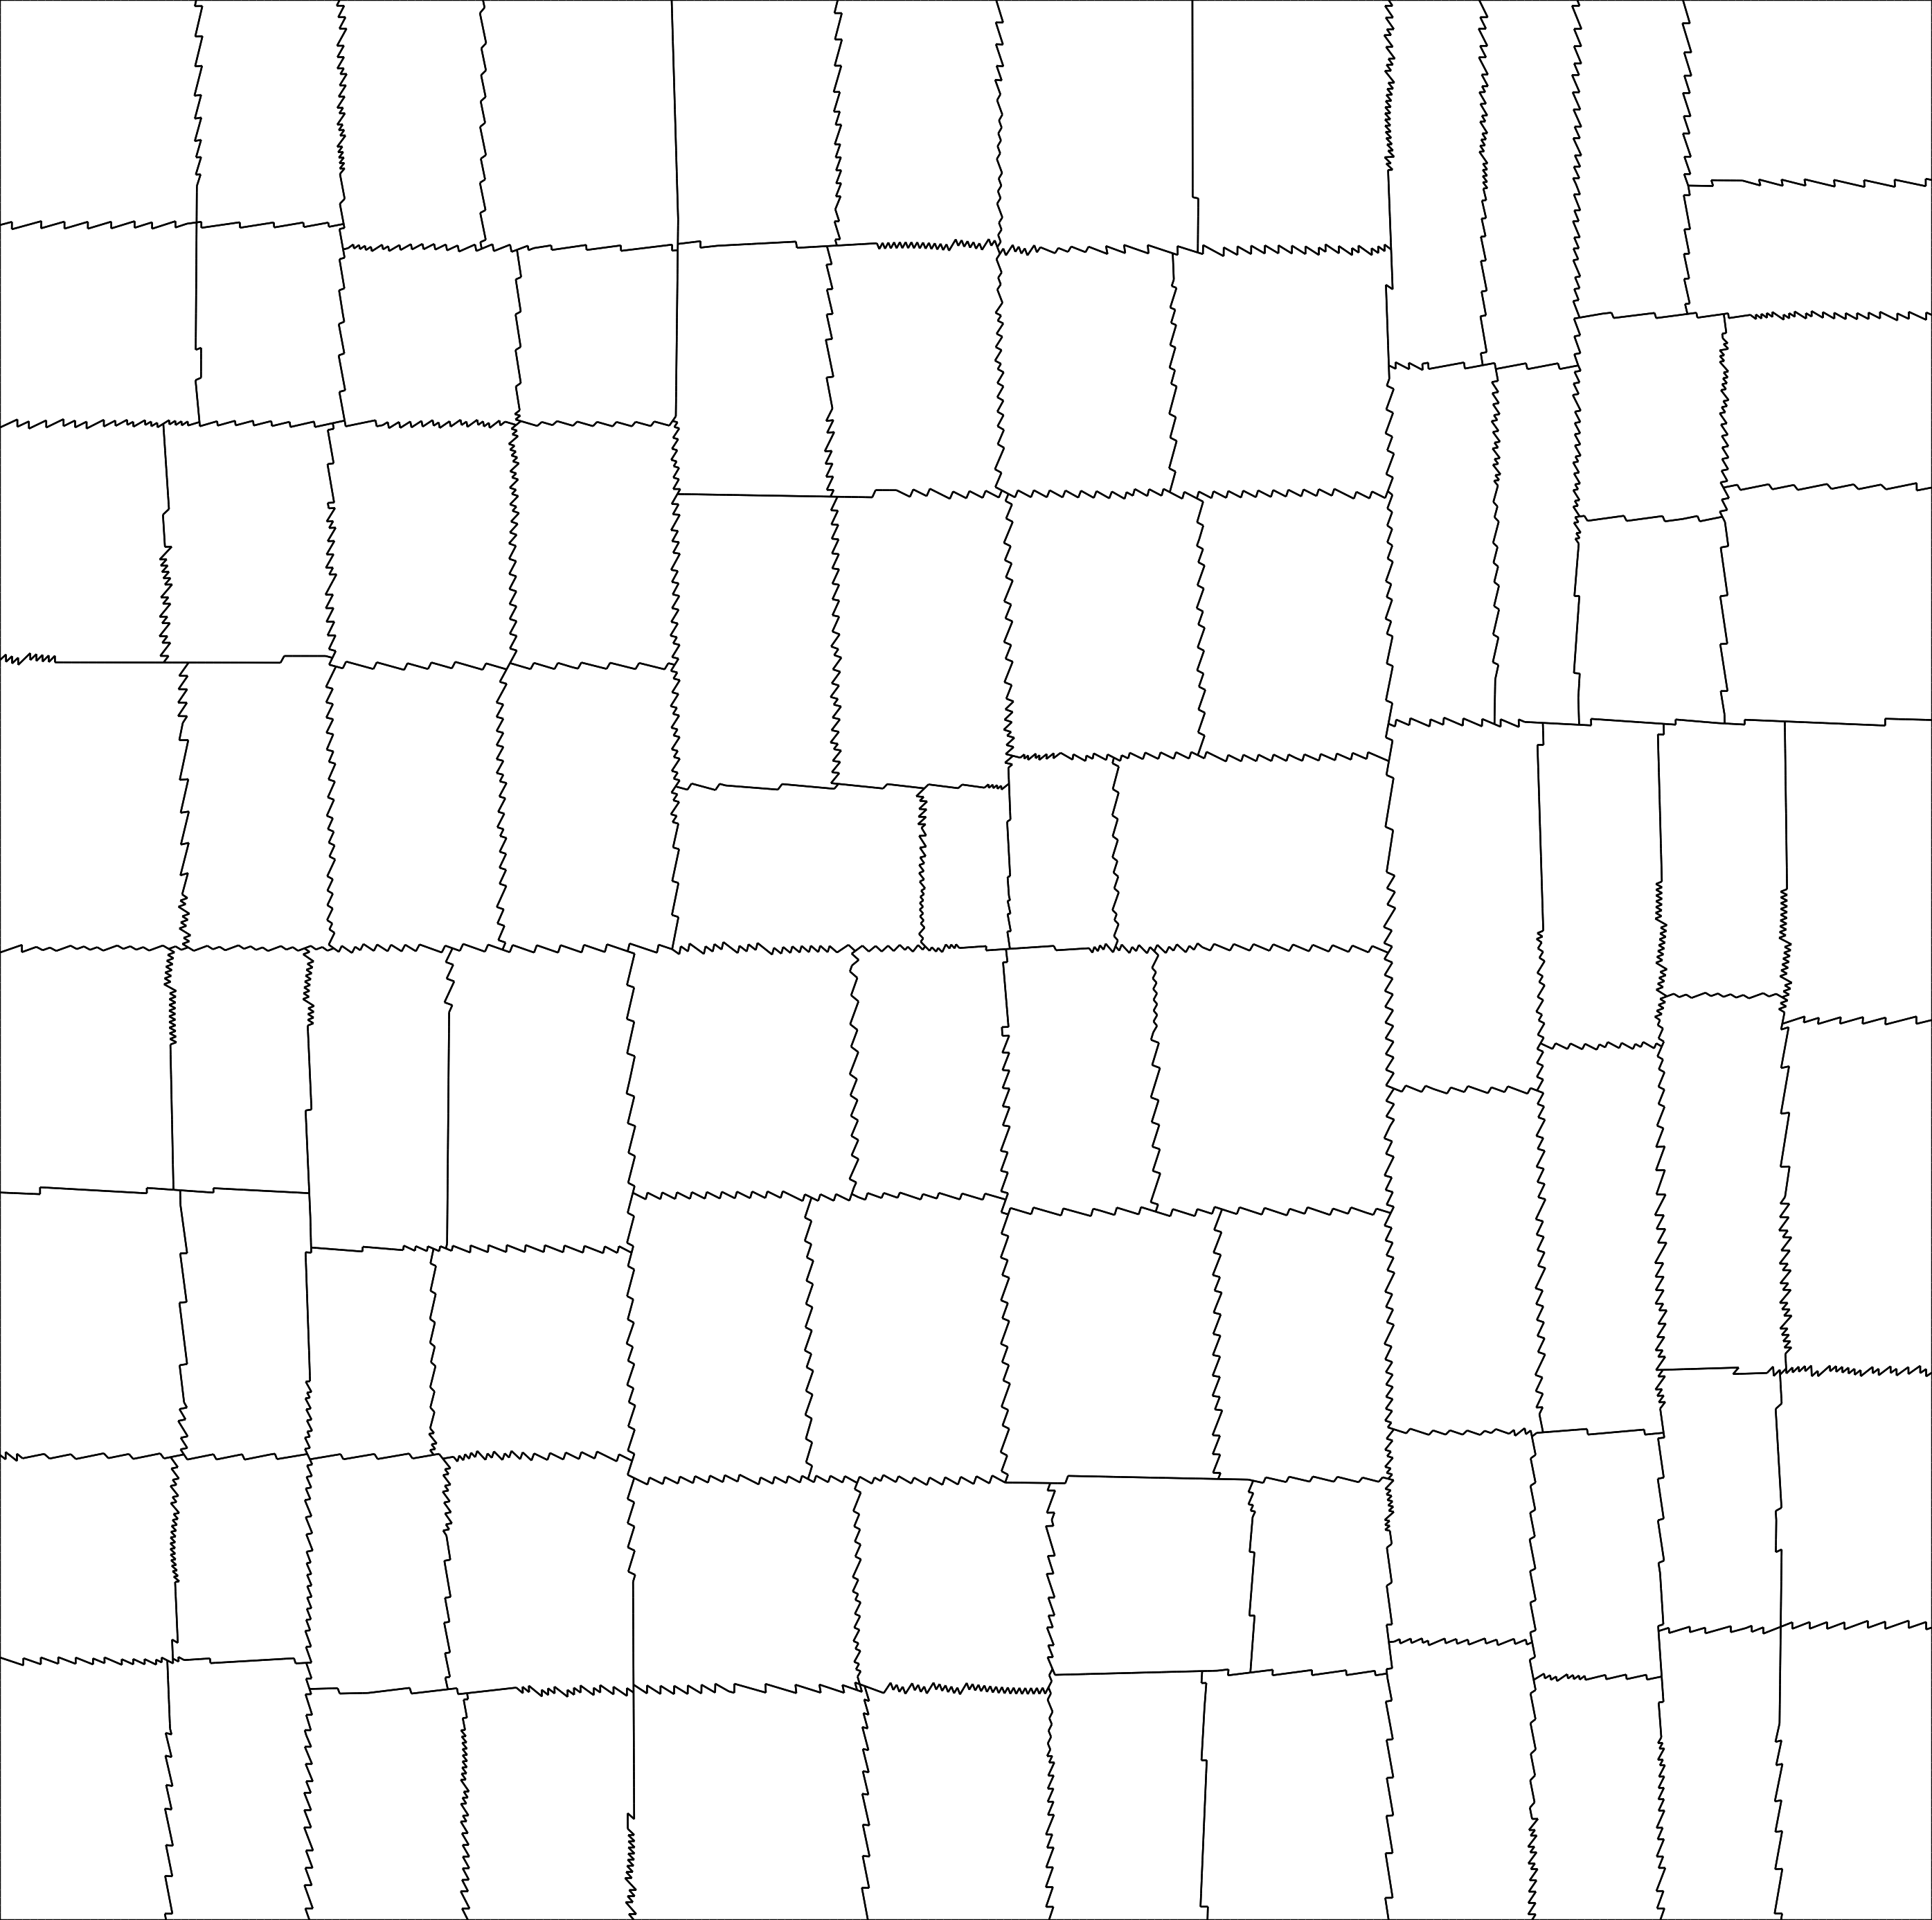
\includegraphics[width=\linewidth]{polygonrtree_91}
        \par\smallskip
        {\small (b) R-tree, 91 agglomerates}
    \end{minipage}

    \par\medskip

    \begin{minipage}[t]{0.47\textwidth}
        \centering
        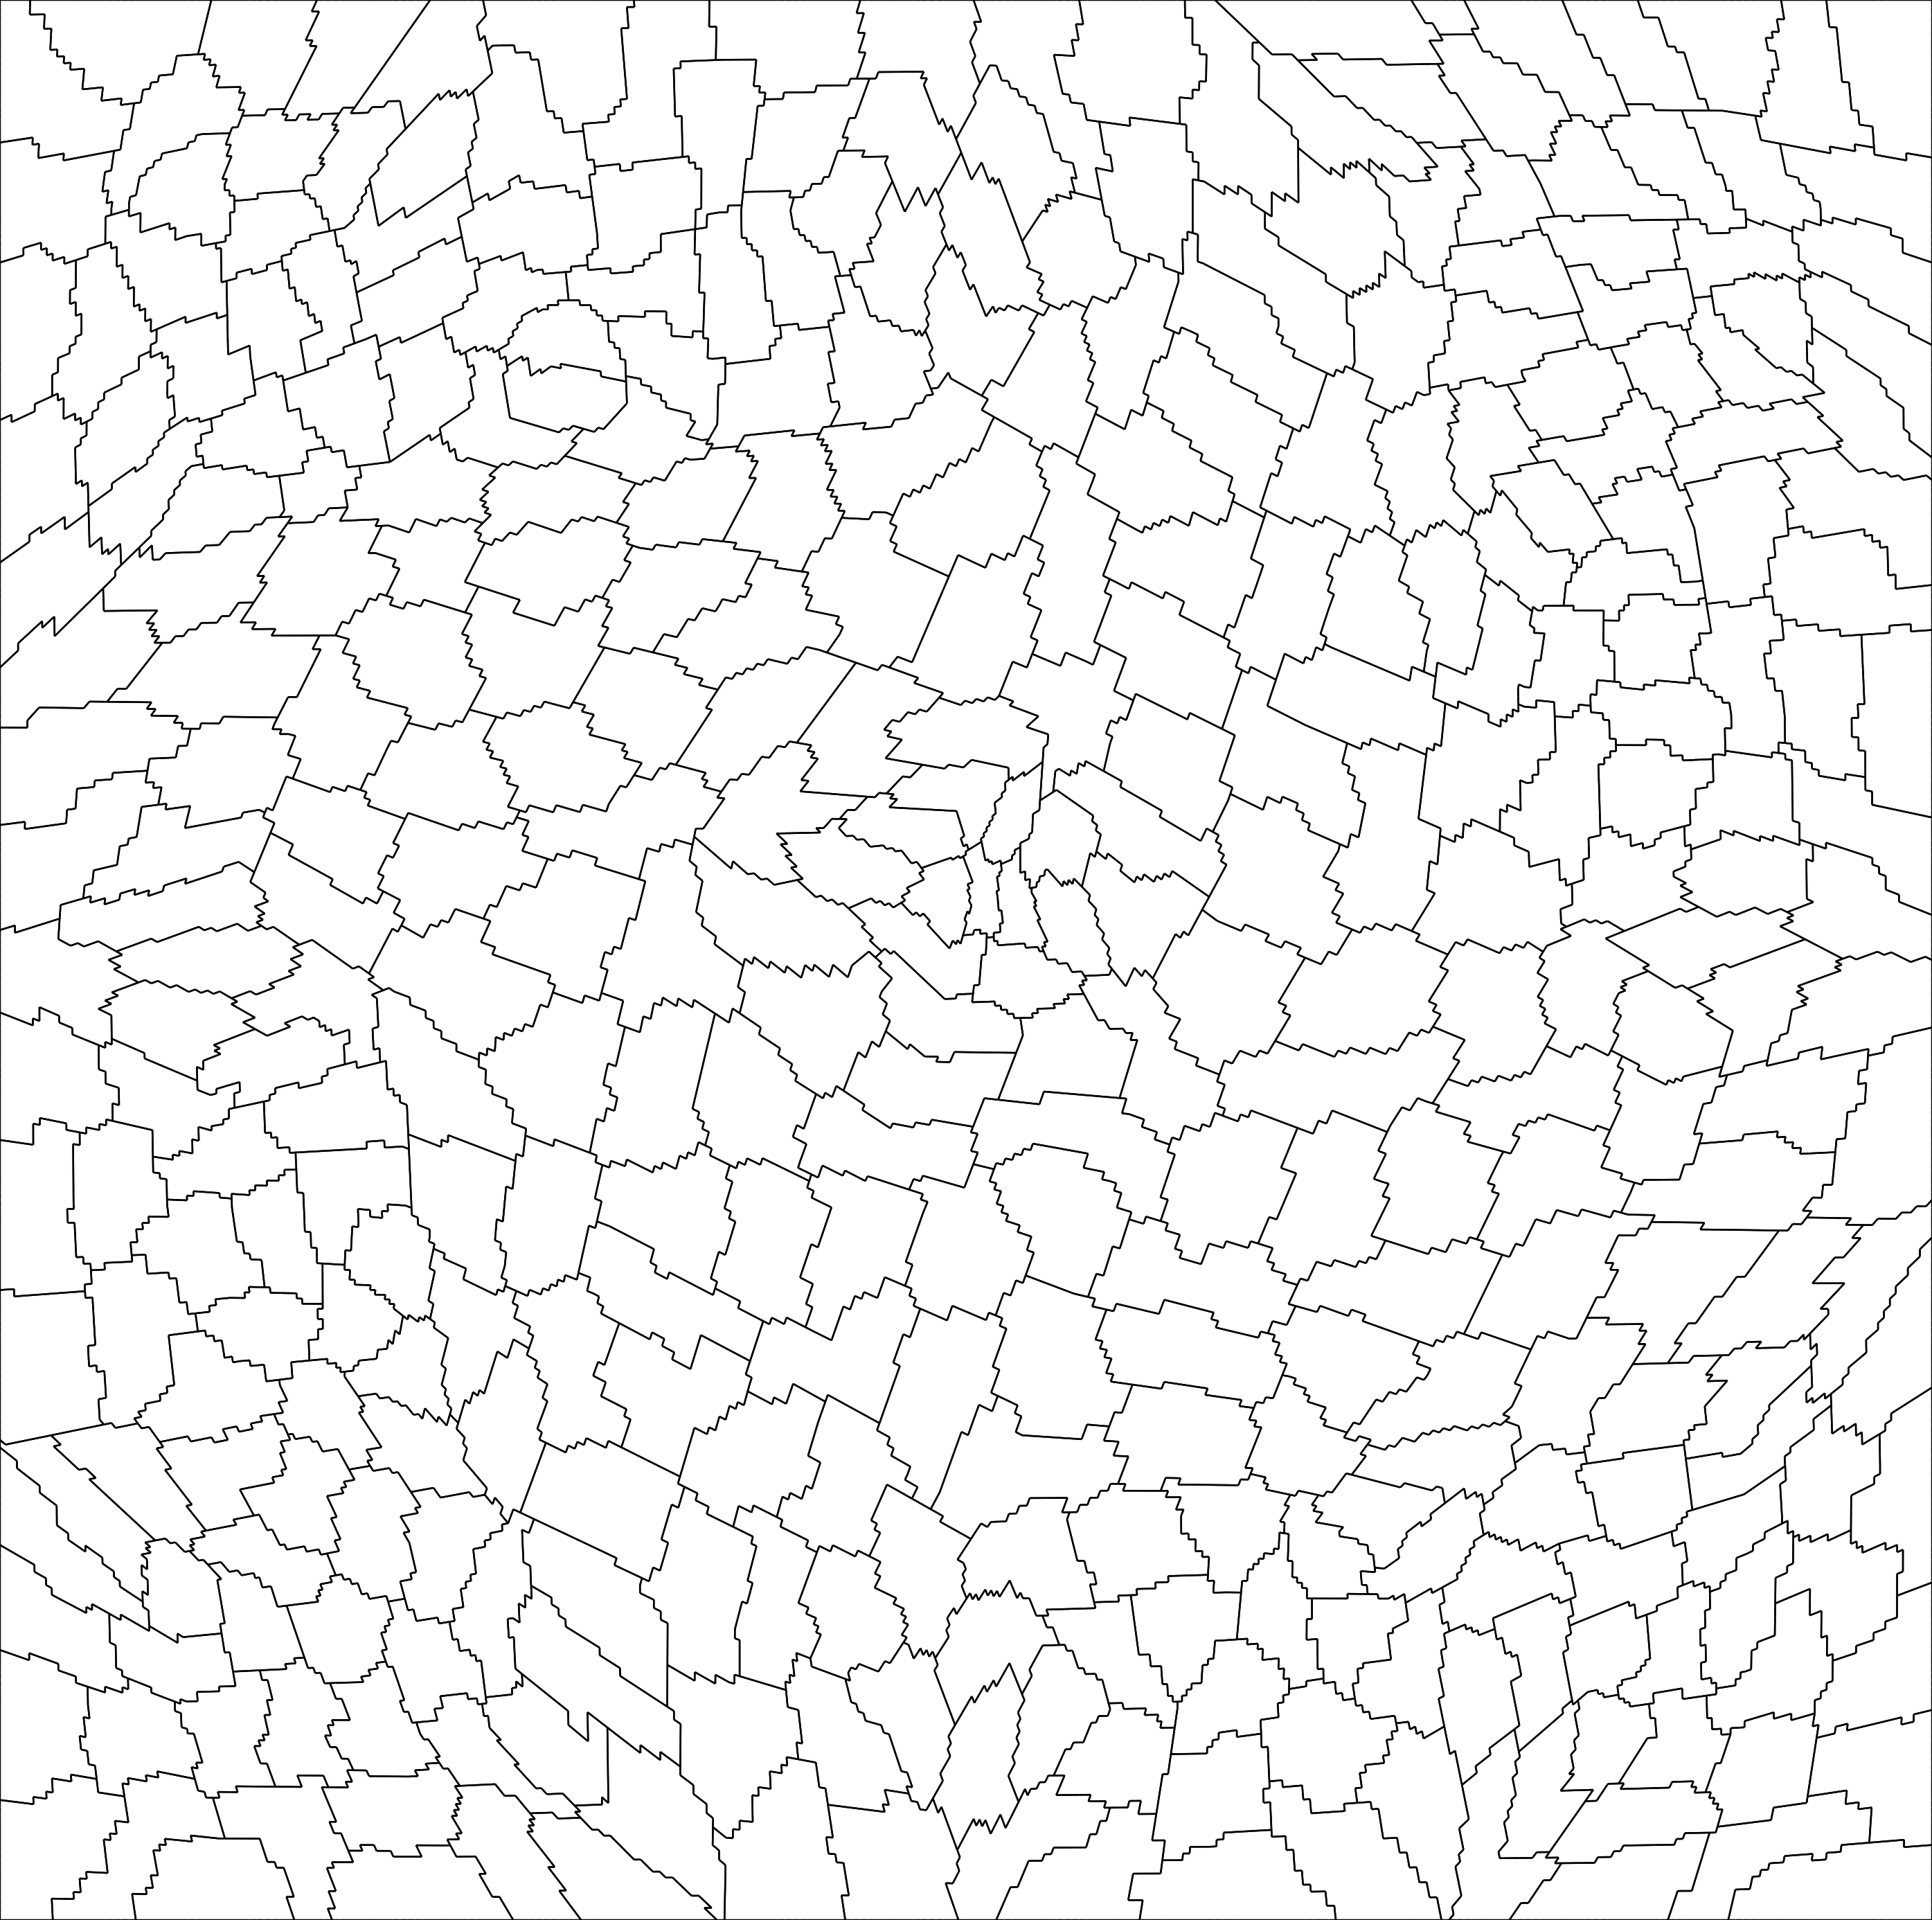
\includegraphics[width=\linewidth]{polygonmetis_364}
        \par\smallskip
        {\small (c) METIS, 364 agglomerates}
    \end{minipage}
    \hfill
    \begin{minipage}[t]{0.47\textwidth}
        \centering
        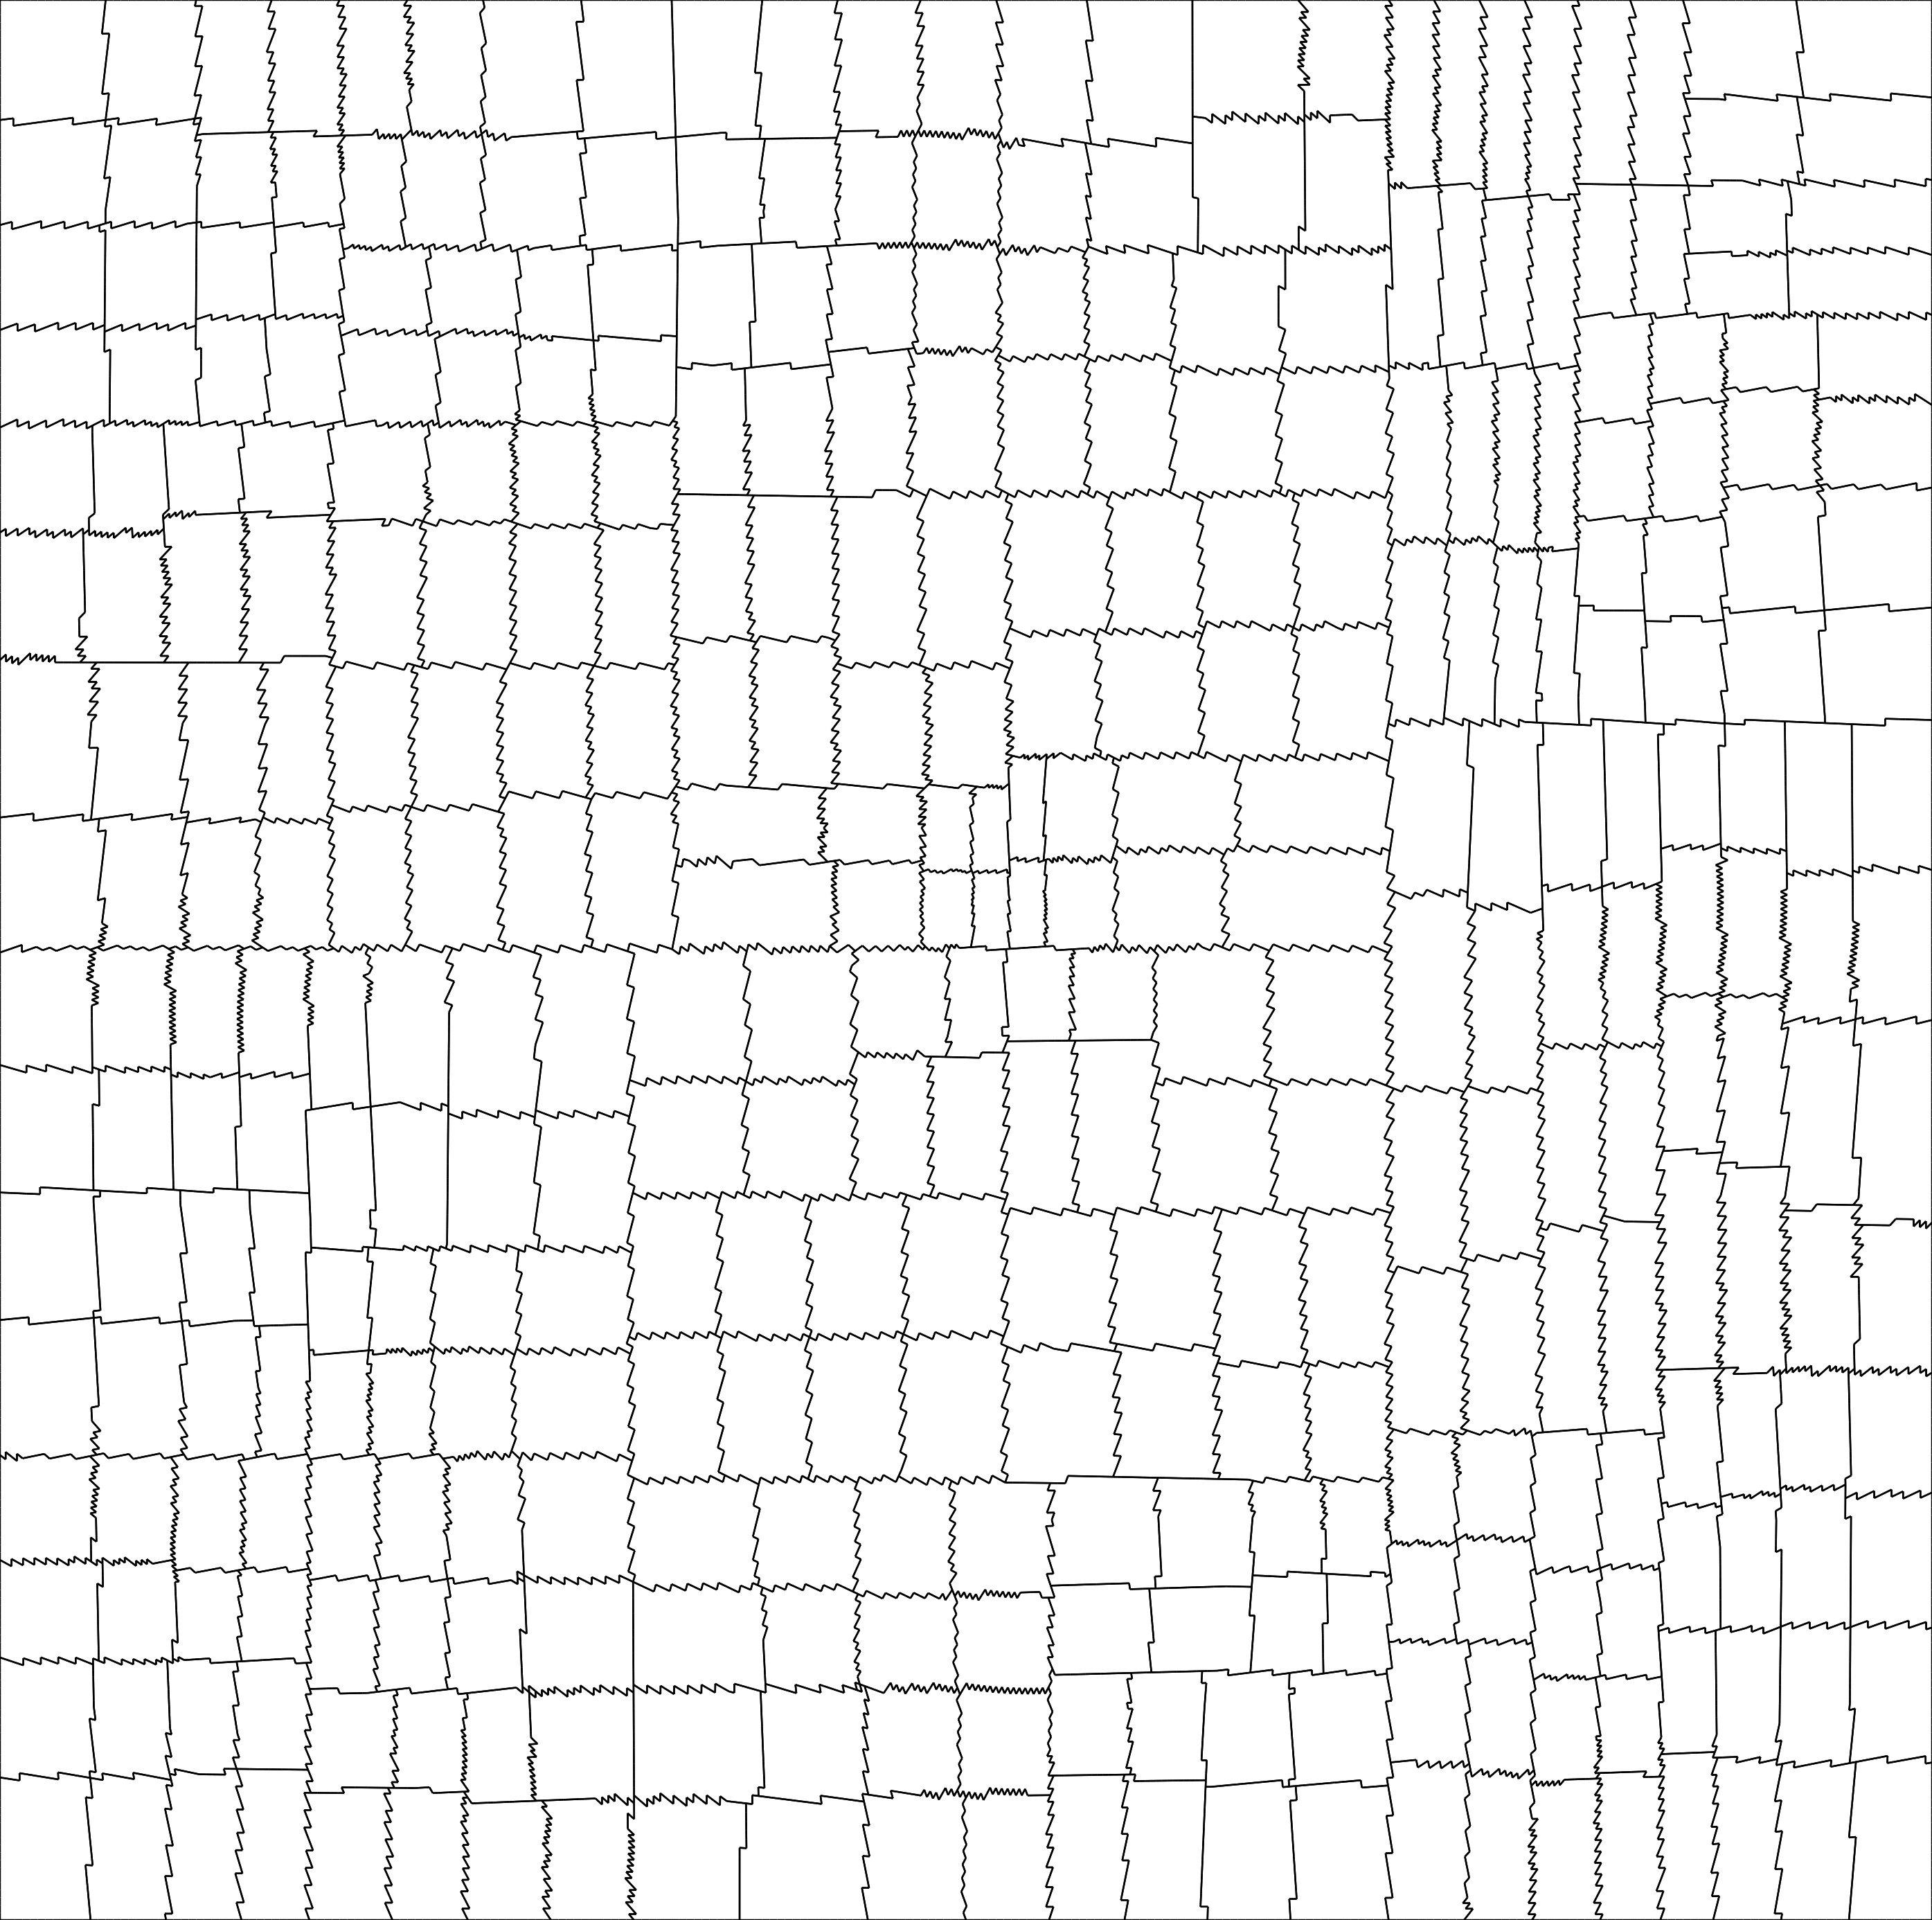
\includegraphics[width=\linewidth]{polygonrtree_364}
        \par\smallskip
        {\small (d) R-tree, 364 agglomerates}
    \end{minipage}

    \caption{Agglomerated polytopic meshes generated from the same fine
        triangulation using METIS and R-tree strategies. The two rows
        correspond to 91 and 364 agglomerates, respectively.}
    \label{fig:code_gallery_meshes}
\end{figure}

Figure~\ref{fig:code_gallery_solutions} shows the numerical solutions obtained
with the two agglomeration strategies. In both cases, the solution is computed
on a mesh containing 91 agglomerates and is subsequently interpolated back
onto the fine mesh for visualization. Although the two methods generate
substantially different agglomerate geometries, they recover the same smooth
solution profile.

\begin{figure}[H]
    \centering

    \begin{minipage}[t]{0.47\textwidth}
        \centering
        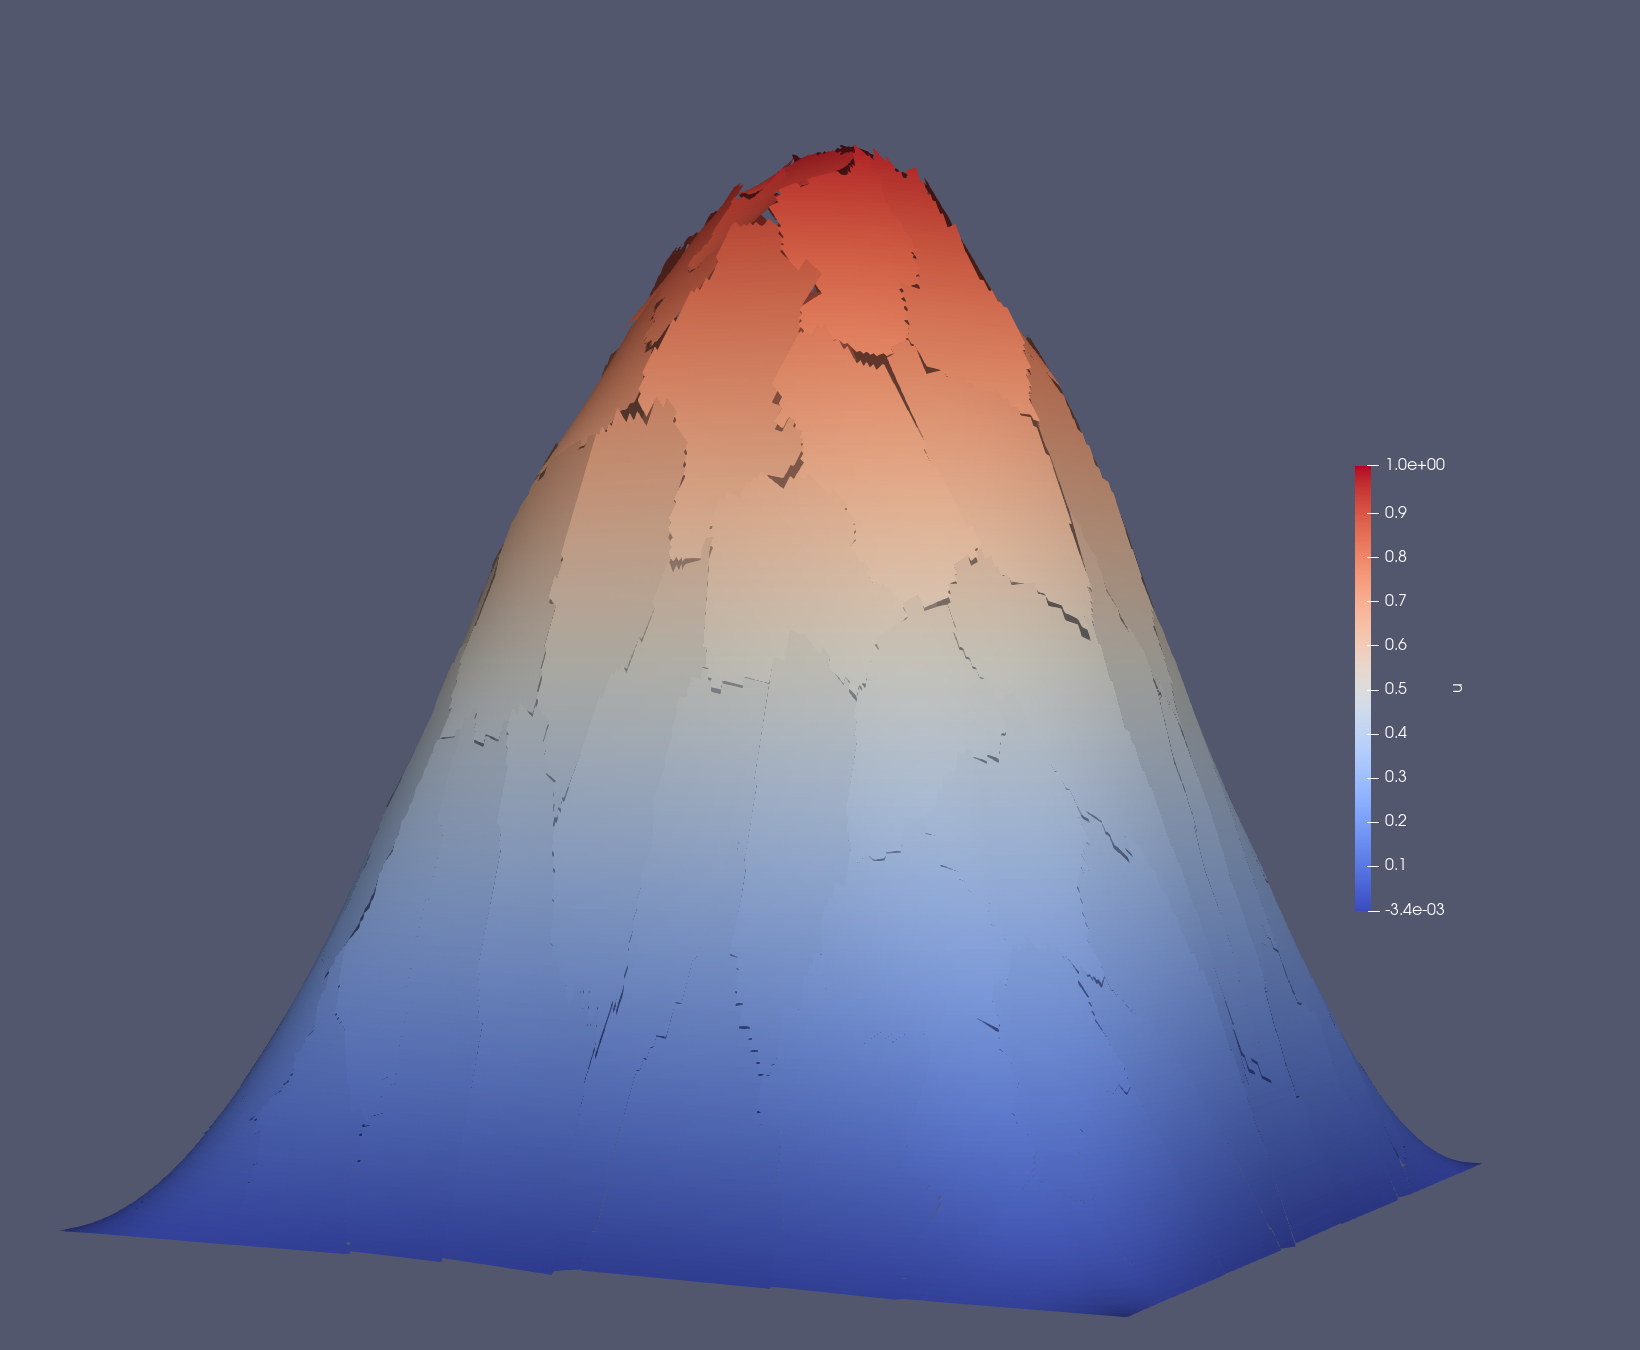
\includegraphics[width=\linewidth]{final_solution_metis}
        \par\smallskip
        {\small (a) METIS agglomeration}
    \end{minipage}
    \hfill
    \begin{minipage}[t]{0.47\textwidth}
        \centering
        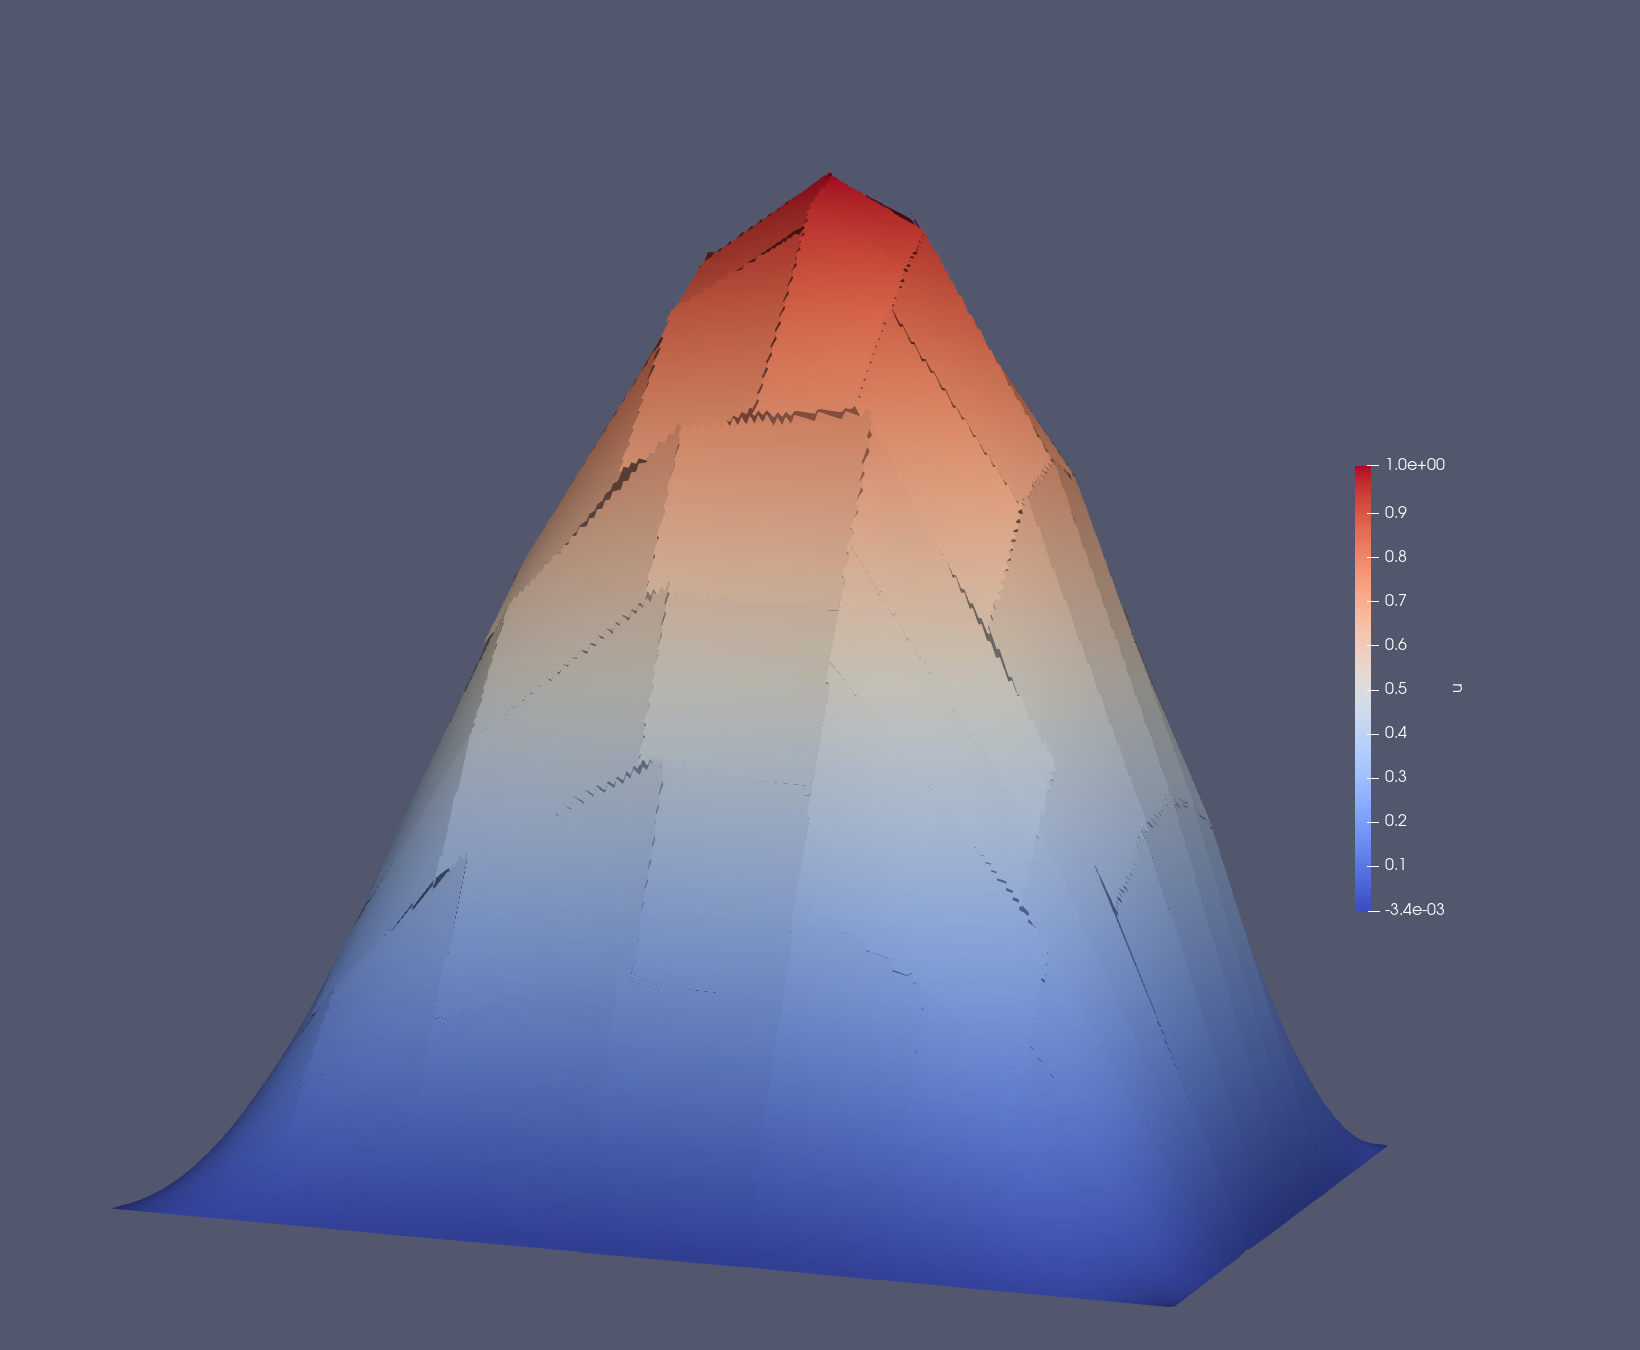
\includegraphics[width=\linewidth]{final_solution_rtree}
        \par\smallskip
        {\small (b) R-tree agglomeration}
    \end{minipage}

    \caption{Numerical solution of the Poisson problem computed on
        91 agglomerates and interpolated onto the fine mesh for
        visualization.}
    \label{fig:code_gallery_solutions}
\end{figure}

%\subsection{{Output and visualization}}
%
%Figure~\ref{fig:agglomeration_comparison} shows polytopic meshes generated
%from the same fine triangulation using METIS and R-tree agglomeration. The two
%strategies produce different element shapes while supporting the same DG
%assembly interface.
%
%\begin{figure}[htbp]
%    \centering
%    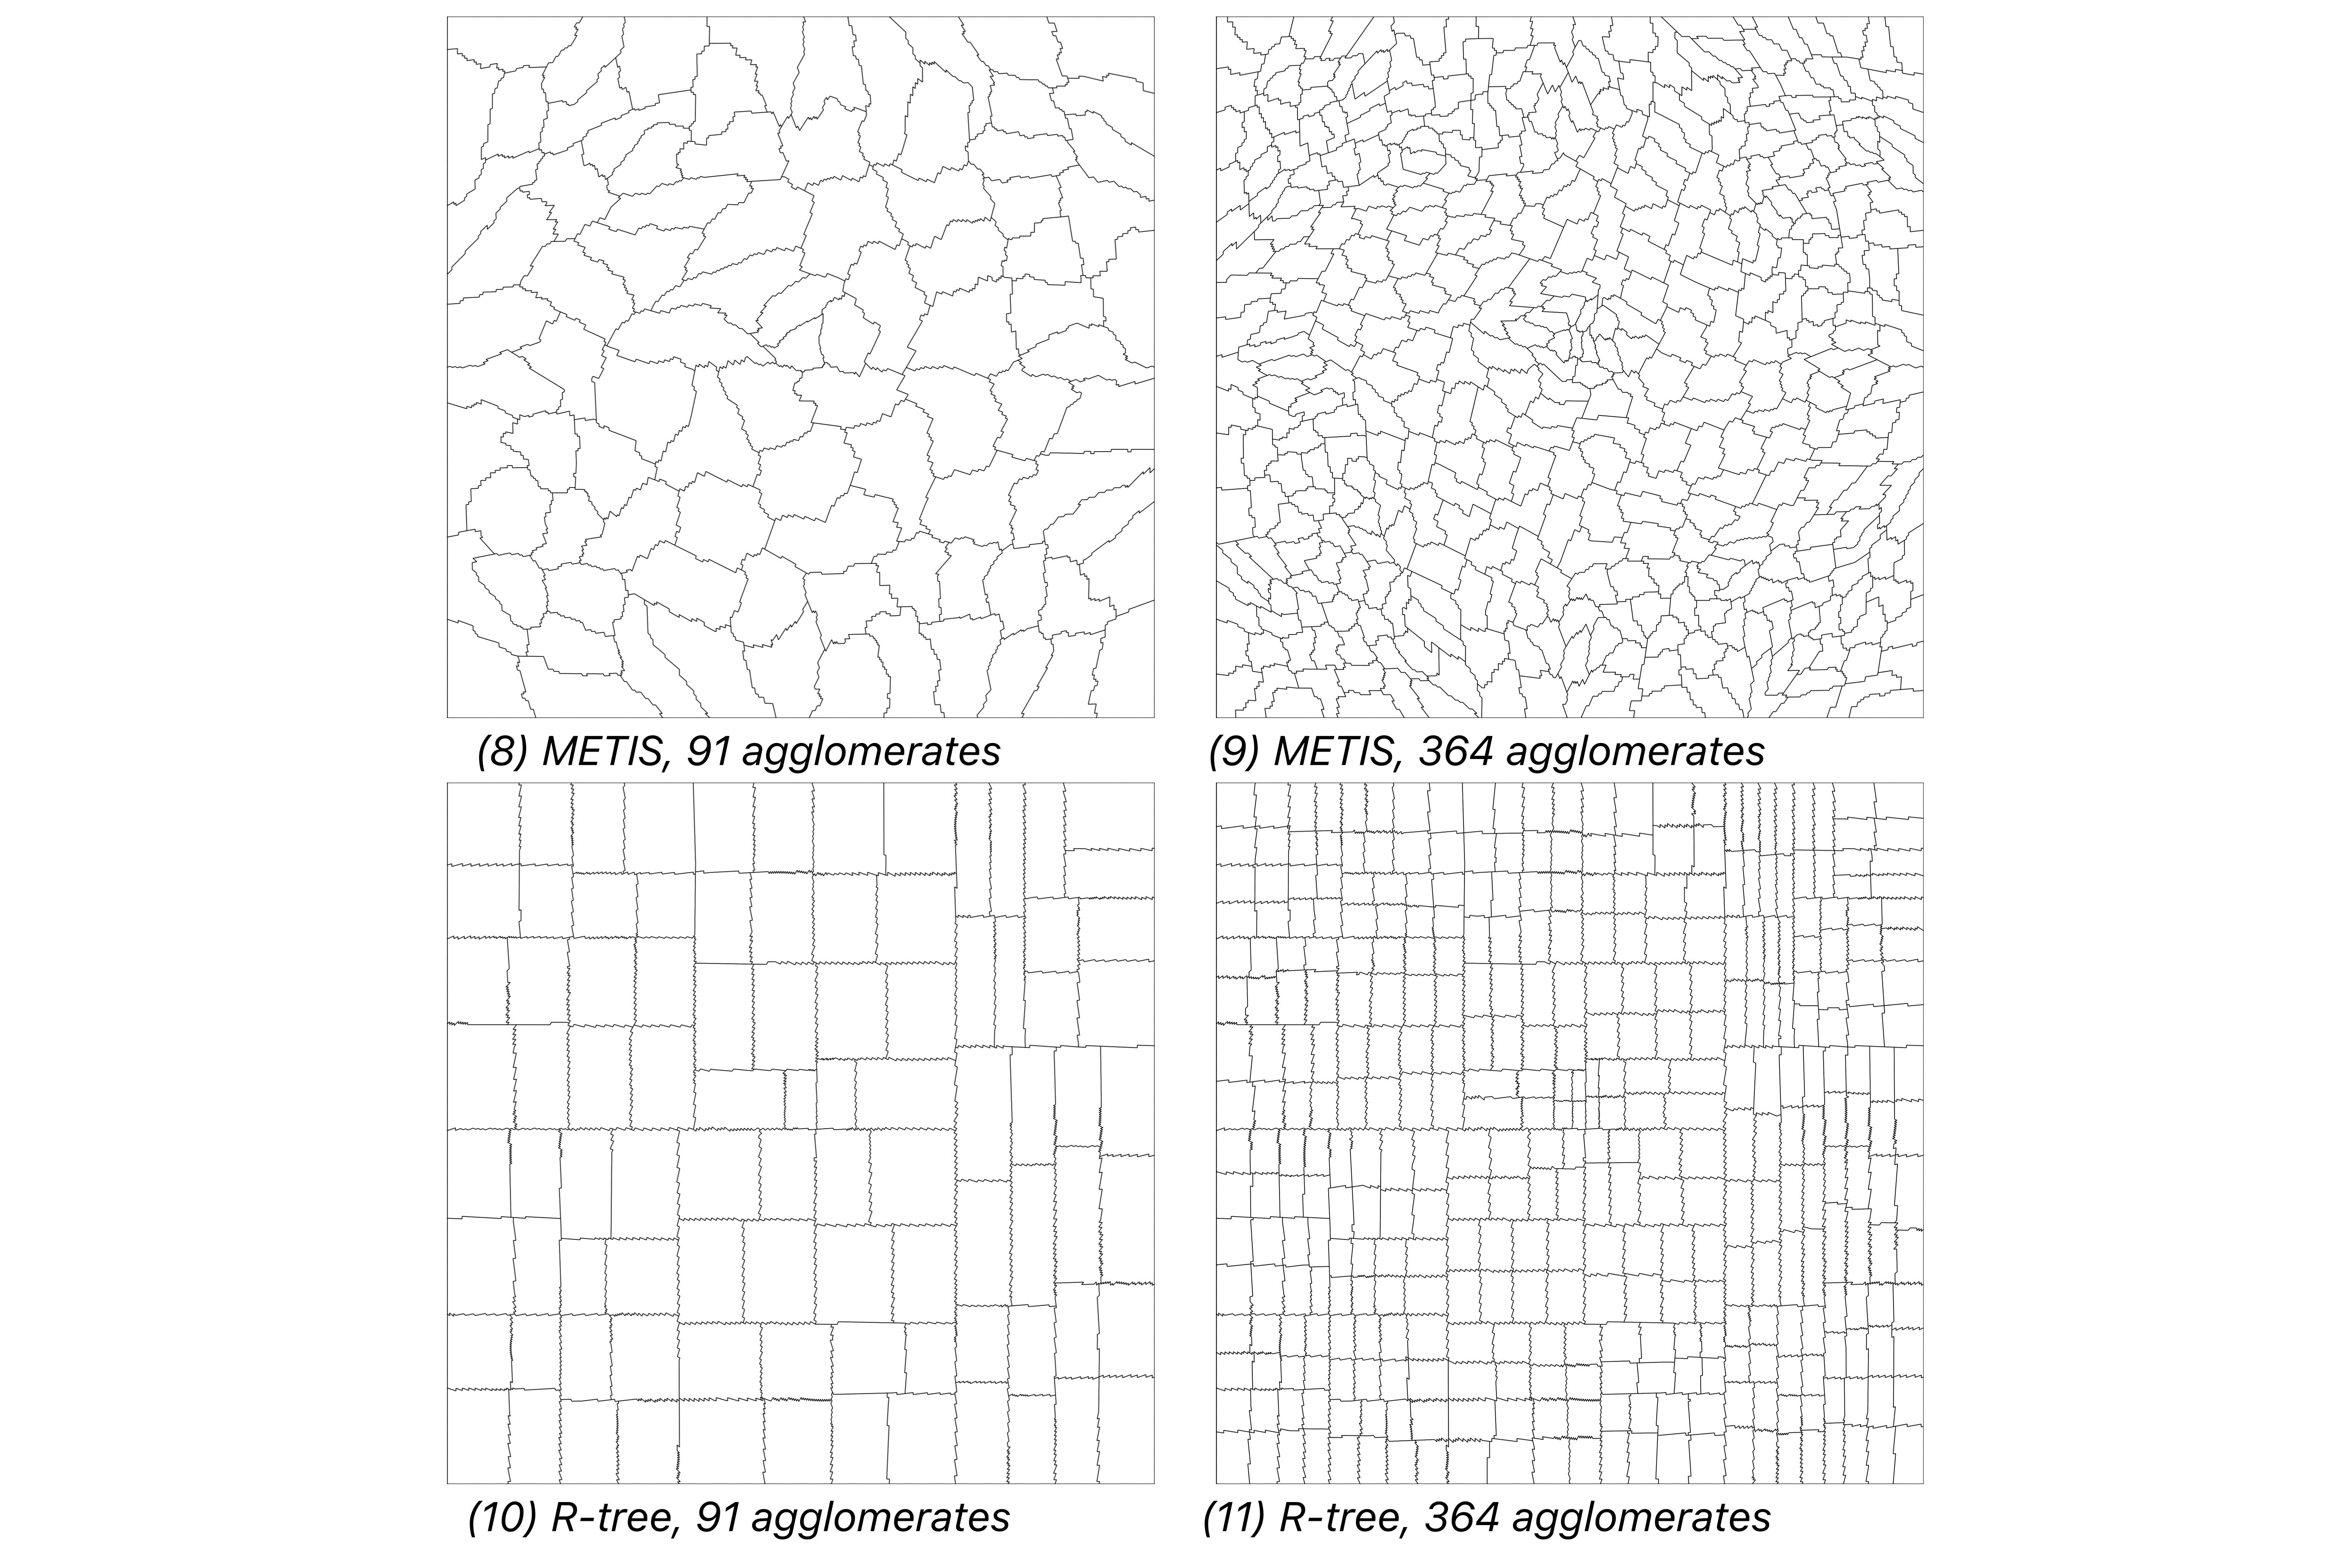
\includegraphics[width=0.88\textwidth]{agglomerates_comparison.png}
%    \caption{Agglomerated meshes generated using METIS and R-tree strategies
%        with 91 and 364 agglomerates. Reproduced from the
%        \href{https://dealii.org/developer/doxygen/deal.II/code_gallery_agglomeration_poisson.html}
%        {official deal.II Code Gallery page}.}
%    \label{fig:agglomeration_comparison}
%\end{figure}
%
%Figure~\ref{fig:p_convergence} reports the reduction of the $L^2$ and broken
%$H^1$ errors under polynomial enrichment for the two agglomeration
%strategies. It provides an end-to-end numerical check of mesh construction,
%DG assembly, solution, and error evaluation.
%
%\begin{figure}[htbp]
%    \centering
%    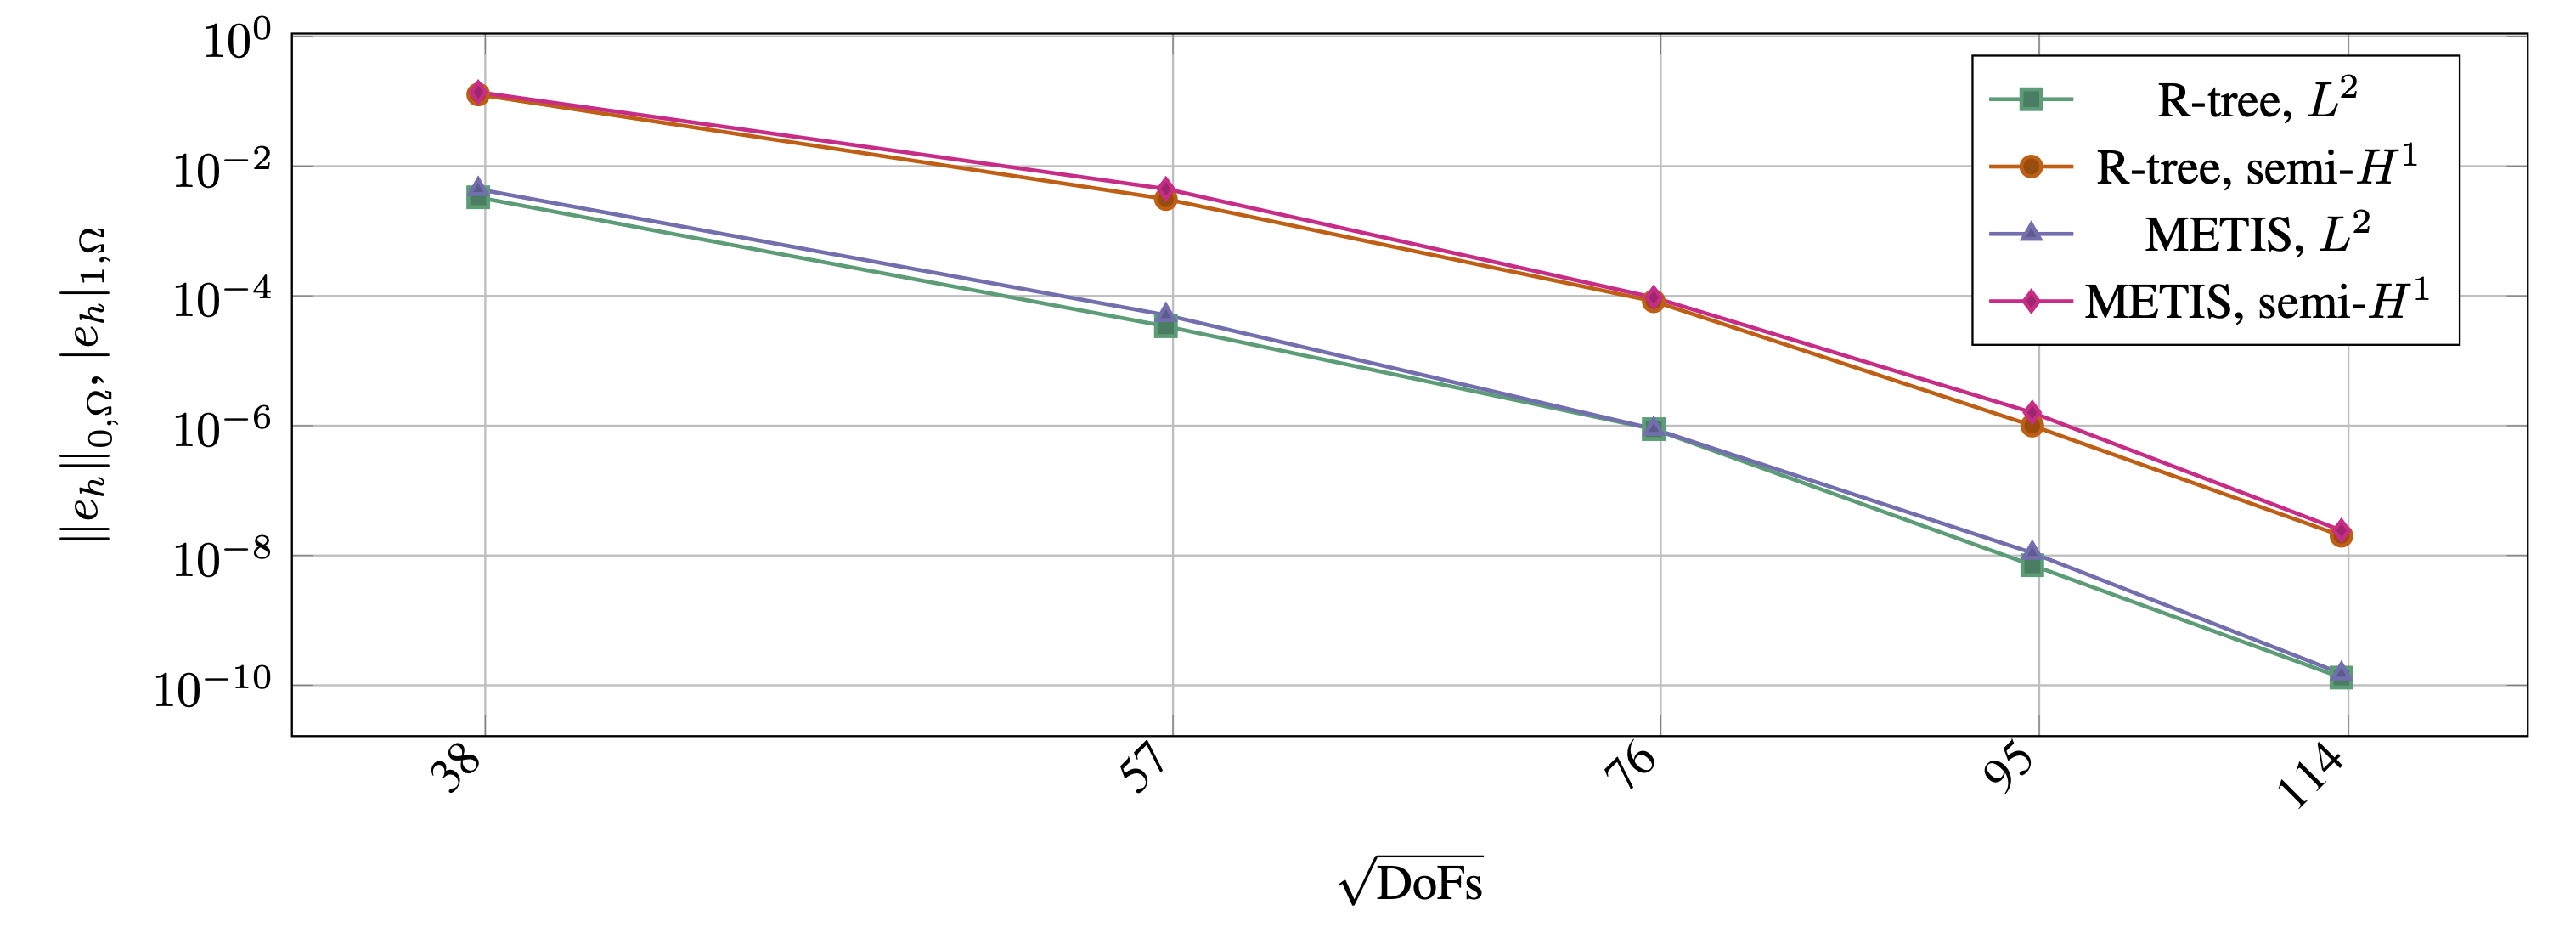
\includegraphics[width=0.92\textwidth]{p_convergence.png}
%    \caption{Convergence of the $L^2$ and broken $H^1$ errors under
%        polynomial enrichment for R-tree and METIS agglomeration. Reproduced
%        from the
%        \href{https://dealii.org/developer/doxygen/deal.II/code_gallery_agglomeration_poisson.html}
%        {official deal.II Code Gallery page}.}
%    \label{fig:p_convergence}
%\end{figure}

% The two figure environments above are intentionally kept separate and can
% be replaced by the two updated Code Gallery figures supplied for the final
% version. Keep the source attribution in the captions after replacement.
\section{{Submission of Polydeal components to the deal.II core library}}
\label{sec:core_pr}

\subsection{{Overview of the submitted framework}}
%\subsection{{Integration of \texttt{Polydeal} functionality into deal.II}}
The core-library submission represents the next step in the integration
process described in D1.7. During this process, the generic components of
\texttt{Polydeal} were separated from application-specific code, adapted to
current deal.II interfaces and coding conventions, and organized for reuse in
different DG applications on agglomerated polygonal and polyhedral meshes.

The resulting contribution was submitted through
\href{https://github.com/dealii/dealii/pull/19891}{deal.II pull request
\#19891}, entitled \emph{Support for agglomeration-based DG
discretizations}. The pull request was opened on June 16, 2026. At the time
of writing, it remains open and is assigned to the deal.II 9.9 release
milestone.


The complete \texttt{Polydeal} project contains functionality beyond the
scope of this pull request, including distributed-memory agglomerated
multigrid components. Pull request \#19891 instead concentrates on the
general-purpose topology, traversal, mapping, quadrature, and finite element
operations that are candidates for inclusion in the deal.II core library.

\subsection{{Main classes and user interface}}

\subsubsection{\texttt{AgglomerationHandler}}

The central class is \texttt{AgglomerationHandler}. Its role for an
agglomerated partition is analogous to the role played by a standard deal.II
\texttt{DoFHandler} on a conventional mesh. It stores the agglomeration
topology, registers collections of fine cells through
\texttt{define\_agglomerate()}, distributes degrees of freedom on the
polytopic mesh through \texttt{distribute\_agglomerated\_dofs()}, and creates
the DG sparsity pattern.

The handler also provides the finite element data required to evaluate cell
terms, boundary terms, and interface contributions. Application code can
therefore assemble a DG operator on agglomerates while continuing to use
standard deal.II matrices, vectors, constraints, and solvers.

\subsubsection{\texttt{AgglomerationAccessor} and
\texttt{AgglomerationIterator}}

The accessor and iterator classes follow the usual deal.II programming
conventions. They allow users to loop over polytopes, retrieve degree-of-
freedom indices, query geometric data and neighboring agglomerates, and
access the faces forming an interface. The bookkeeping associated with the
underlying fine cells is hidden from the application.

The resulting loop has the same overall structure as a standard deal.II cell
loop:
\begin{lstlisting}[caption=Iteration over agglomerated elements]
for (const auto &polytope : handler.polytope_iterators())
{
  cell_matrix = 0;
  cell_rhs    = 0;
  polytope->get_dof_indices(local_dof_indices);

  // Evaluate shape functions and assemble cell and face terms.
  // Distribute the local contributions to the global system.
}
\end{lstlisting}

\subsubsection{\texttt{CellsAgglomerator} and \texttt{MappingBox}}

\texttt{CellsAgglomerator} constructs agglomerates using a packed
Boost.Geometry R-tree. Selecting a level of the tree groups fine cells into a
coarser partition. Different tree levels consequently define a hierarchy of
agglomerated meshes suitable for subsequent multilevel developments.

\texttt{MappingBox} is an agglomeration-aware Cartesian mapping. For each agglomerate, it maps the reference cell to the associated axis-aligned bounding box. The finite element basis on the physical agglomerate is obtained by restricting the basis defined on this box. The mapping is used internally to transform quadrature points to reference coordinates and to evaluate shape functions.

\subsection{{Main design choices}}

\subsubsection{Master and slave cells}

Each agglomerate is a collection of cells of the original triangulation. One
cell is selected as the \emph{master} and carries the degrees of freedom of
the complete agglomerate. The remaining \emph{slave} cells carry no
independent degrees of freedom and are assigned \texttt{FE\_Nothing}. An
internal hp structure automates this assignment. This design makes it
possible to reuse the existing deal.II \texttt{DoFHandler} infrastructure
without assigning a separate finite element space to every constituent cell.

\subsubsection{Quadrature on an agglomerate}

An arbitrary polytope does not generally have a standard reference-cell
quadrature rule. The submitted implementation constructs its volume
quadrature by collecting standard quadrature rules from all fine cells in the
agglomerate. The physical points and weights are retained, and the points are
also mapped to the bounding-box reference coordinates for shape-function
evaluation. Thus, if $K$ is the union of fine cells $K_i$, integration is
performed as
\begin{equation}
    \int_K f\,\mathrm{d}x = \sum_i \int_{K_i} f\,\mathrm{d}x.
\end{equation}

\subsubsection{Interfaces between neighboring agglomerates}

The interface between two neighboring polytopes may contain several faces of
the original triangulation. It is therefore represented as the collection of
standard deal.II faces separating the two agglomerates. DG jumps, averages,
and flux terms can then be assembled face by face using the existing deal.II
finite element evaluation machinery.

\subsection{{Typical workflow}}

The main steps exposed by the submitted interface are shown below. The
listing is schematic; the selection of fine cells can be supplied by the
R-tree agglomerator or by an application-specific partitioning strategy.

\begin{lstlisting}[caption=Schematic workflow for an agglomerated DG method]
GridTools::Cache<dim> cache(tria, mapping);
AgglomerationHandler<dim> handler(cache);

for (const auto &cells : cells_per_agglomerate)
  handler.define_agglomerate(cells);

FE_DGQ<dim> fe(degree);
handler.distribute_agglomerated_dofs(fe);

DynamicSparsityPattern dsp;
handler.create_agglomeration_sparsity_pattern(dsp);

for (const auto &polytope : handler.polytope_iterators())
{
  const auto &values = handler.reinit(polytope);
  polytope->get_dof_indices(local_dof_indices);
  // Assemble volume, boundary, and interface terms.
}
\end{lstlisting}

The important point is that the application works with polytopes through
handler and iterator interfaces, whereas the original triangulation remains
available for standard geometric operations.

\subsection{{Tests and current status}}

Pull request \#19891 includes initial regression tests covering different
parts of the proposed infrastructure:
\begin{itemize}
    \item \texttt{3DRtree} checks R-tree extraction and agglomeration in
          three dimensions;
    \item \texttt{fe\_space\_on\_bbox} checks finite element evaluation and
          collected quadrature on bounding boxes in two and three dimensions;
          and
    \item \texttt{poisson\_sanity\_check\_01} checks the combined degree-of-
          freedom, sparsity, quadrature, and DG assembly workflow on an
          agglomerated Poisson problem.
\end{itemize}

The pull request is a submitted proposal rather than
an accepted part of deal.II. Maintainer review and completion of the upstream
continuous-integration checks remain necessary. Because the contribution is
substantial, it may be divided into smaller pull requests if this is preferred
during review. Such a division would change the integration procedure but not
the functionality described above.


\section{{Conclusion}}
\label{sec:conclusion}

The agglomeration-based Poisson program is now publicly available through the
official deal.II Code Gallery. 

The reusable agglomeration infrastructure has been submitted separately to
the deal.II core library through pull request \#19891. The proposal provides
handler, iterator, accessor, mapping, quadrature, degree-of-freedom,
sparsity, and R-tree agglomeration components for DG methods on polygonal and
polyhedral meshes. At the reporting date, the core pull request remains open and is awaiting maintainer review. Its eventual upstream integration is the next software step.



\begin{thebibliography}{10}

\bibitem[Cangiani et al., 2014]{polyDG}
Andrea Cangiani, Emmanuil Georgoulis, and Paul Houston,
"$hp$-Version discontinuous Galerkin methods on polygonal and polyhedral
meshes," \emph{Mathematical Models and Methods in Applied Sciences},
vol.~24, no.~10, pp.~2009--2041, 2014.

\bibitem[Antonietti et al., 2013]{Antoniettihp}
Paola F. Antonietti, Stefano Giani, and Paul Houston,
"$hp$-Version composite discontinuous Galerkin methods for elliptic problems
on complicated domains," \emph{SIAM Journal on Scientific Computing},
vol.~35, pp.~A1417--A1439, 2013.

\bibitem[Feder et al., 2025]{FEDER2025113773}
Marco Feder, Andrea Cangiani, and Luca Heltai,
"R3MG: R-tree based agglomeration of polytopal grids with applications to
multilevel methods," \emph{Journal of Computational Physics}, vol.~526,
113773, 2025.

\bibitem[Feder and Africa, 2026]{FederAfrica2026}
Marco Feder and Pasquale Claudio Africa,
``An agglomeration-based multigrid solver for the discontinuous Galerkin
discretization of cardiac electrophysiology,''
\emph{arXiv preprint arXiv:2602.16312}, 2026.
\url{https://arxiv.org/abs/2602.16312}.

\bibitem[Karypis and Kumar, 1998]{METIS}
George Karypis and Vipin Kumar,
"A fast and high quality multilevel scheme for partitioning irregular
graphs," \emph{SIAM Journal on Scientific Computing}, vol.~20,
pp.~359--392, 1998.

\end{thebibliography}

\label{MyLastPage}

\end{document}

%%% Local Variables:
%%% mode: LaTeX
%%% TeX-master: t
%%% End:
